% !TeX spellcheck = en_US

\chapter{Concept Description}

	uFixit is a platform on which user can get manuals that help them repair things. It does not matter from which manufacturer it comes, it works with all products of either brand. There is only one minor constraint: The part has to be fixable.
	
	\begin{figure}[H]
		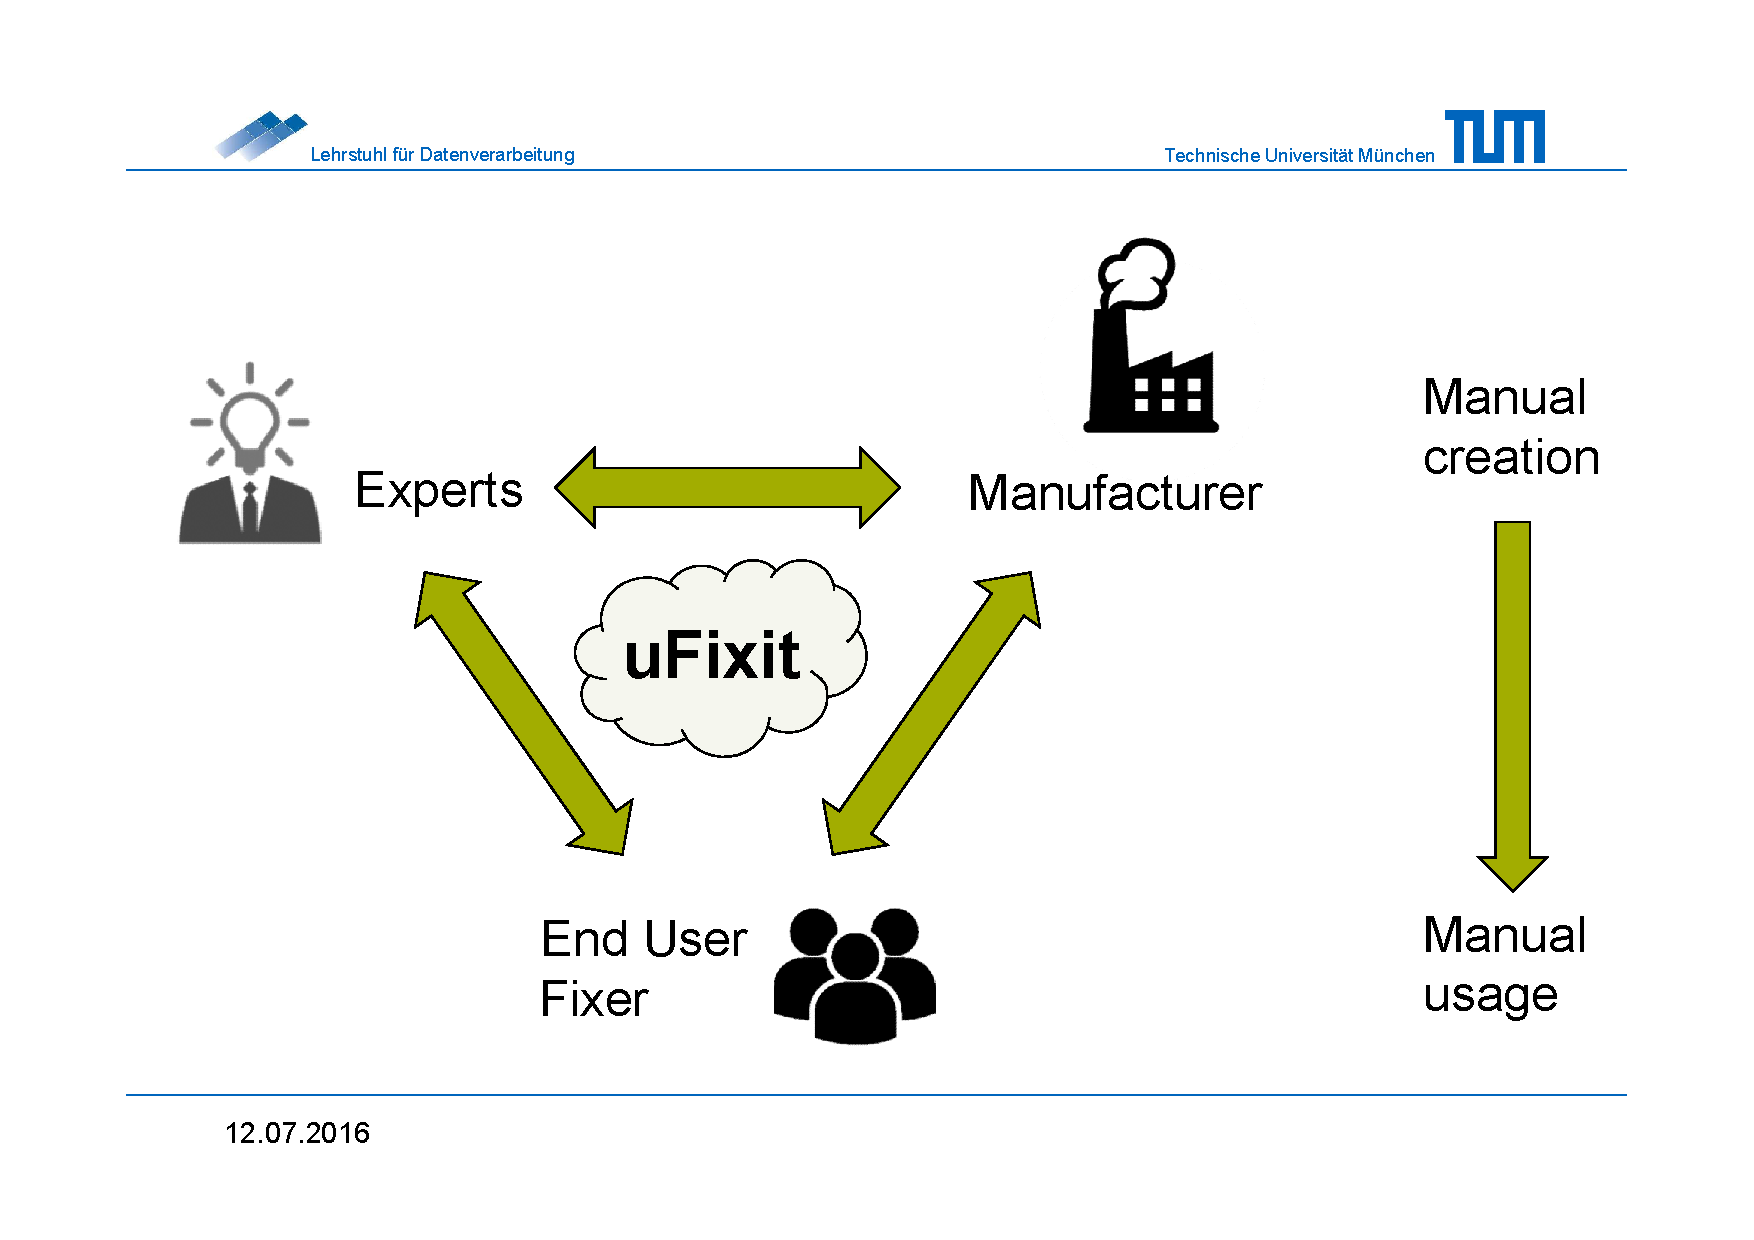
\includegraphics[width=\textwidth, trim=0cm 3cm 0cm 4cm, clip]{../images/involved-parties.pdf}
		\centering
		\caption{Parties involved in the uFixit environment}
		\label{fig:involved-parties}
	\end{figure}

	As one can see in \autoref{fig:involved-parties}, \textbf{Experts} and \textbf{Manufacturers} create the manuals, whereas \textbf{Fixers} use them on their own device. An Expert is a person that has the same equipment as the end user, but does create manuals. He will not have special training or software to do so. Manufacturers on the other side have detailed information and models of their products and therefore can develop high quality instruction steps with animations and extensive highlightings.
	
	After describing how the instructions inside a manual will look like, we discuss how uFixit helps experts as well as manufacturers in creating the best possible manuals for the end user. For the conclusion of this chapter we will have a look at how the experts will be motivated to create content for our platform.


	\section{Instructions format}
	\label{sec:instr-format}
	
		Every manual will be separated into several individual steps. The first step is always the diagnosis because to do the repair itself, we do need to know what is broken. While holding the defective part into the FOV of the camera, uFixit will try to match it to a internal database. If this succeeds, the next step is to get the right manual and the suitable tools.
		
		
		After this preparation phase, the actual repair process begins. Each of the steps will ask the user to perform a specific task to fulfill. Subsequently the manual must transition to the next step. There are a few different possibilities:
		
		\begin{itemize}
			\itemsep0em
			\item The AR device constantly watches the fixer while performing the task. Due to sophisticated algorithms, the application can detect when it is finished and will automatically jump to the next one.
			\item Ideally the used device has a microphone built in. With that, the fixer simply can issue a voice command.
			\item Although it is more of a feature to jump to a specific step in the tutorial, forward and backward buttons will be provided on screen for easy access.
		\end{itemize}
		
		\begin{figure}[H]
			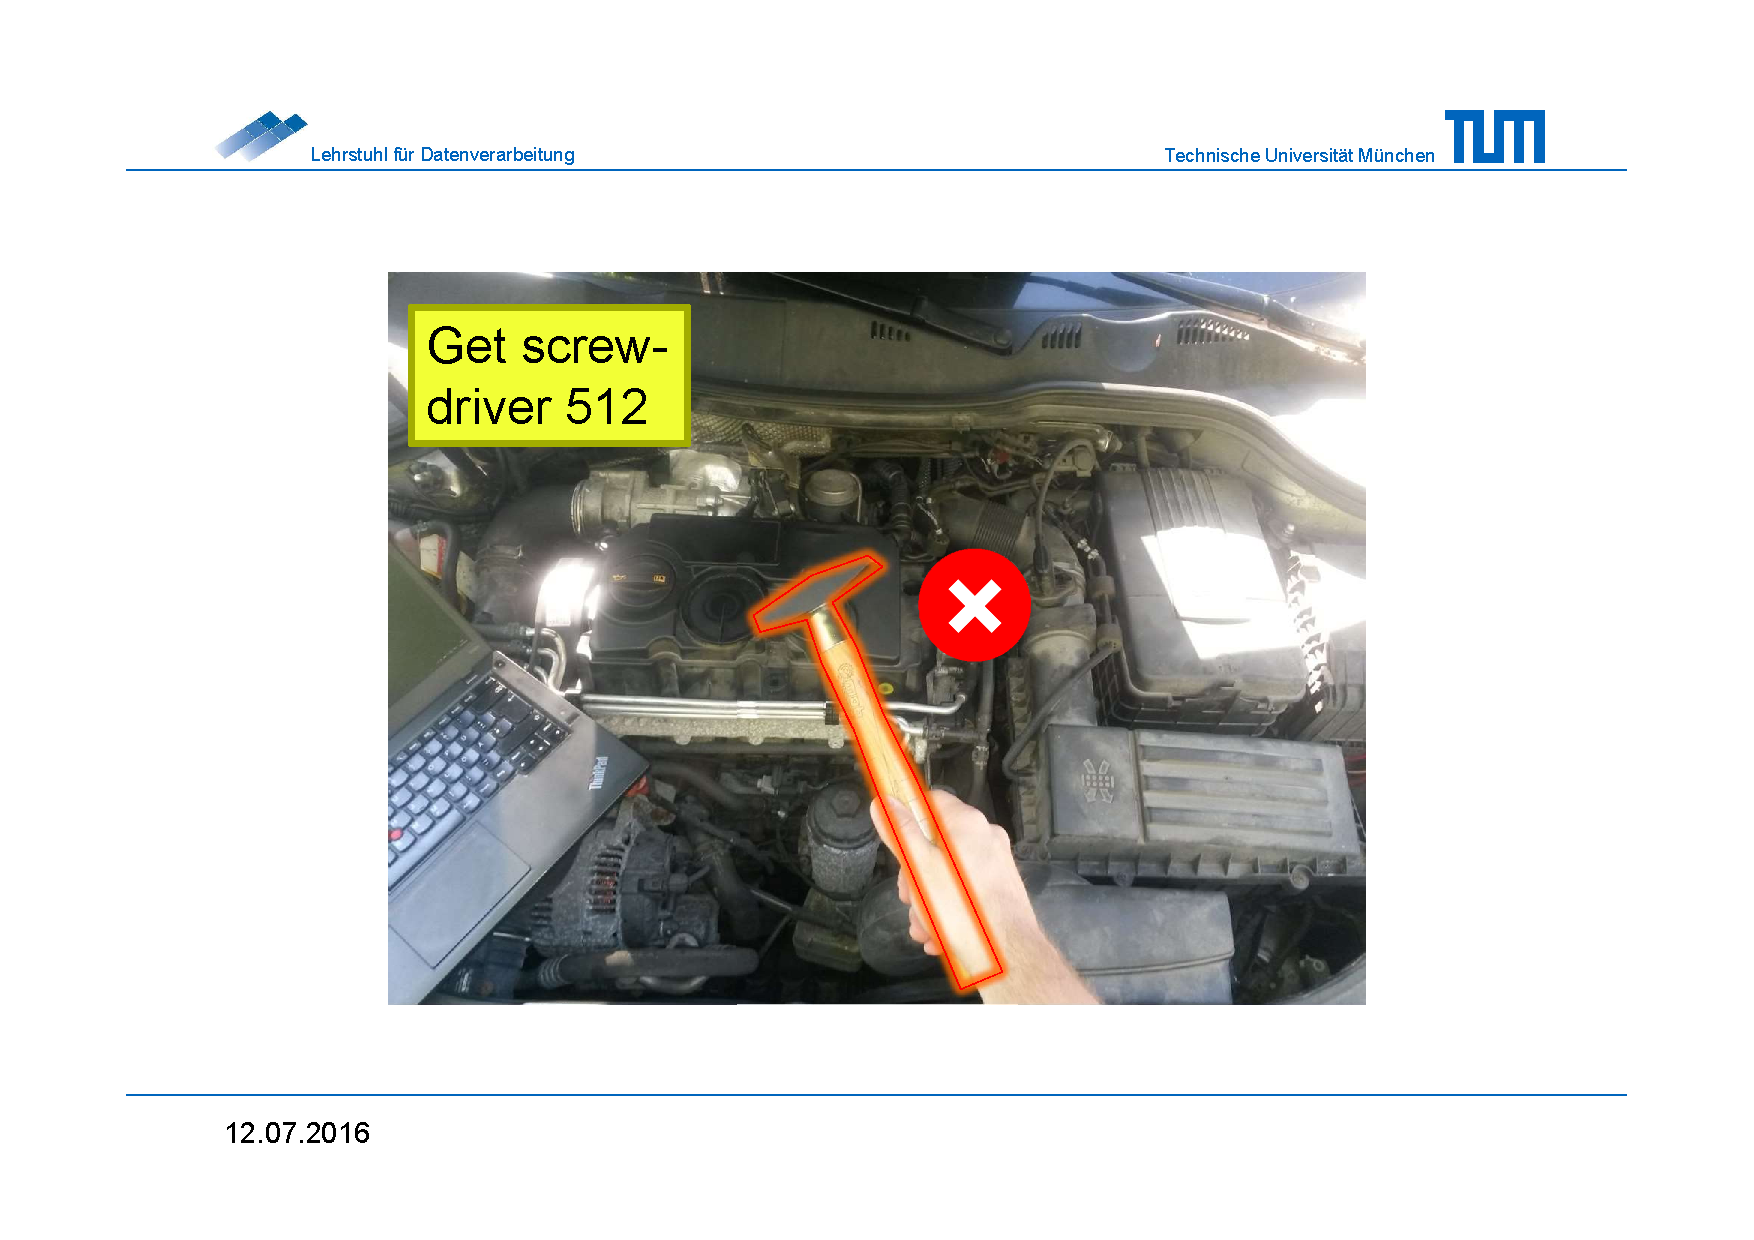
\includegraphics[width=\textwidth, trim=4cm 3cm 4cm 4cm, clip]{../images/instr-hammer.pdf}
			\centering
			\caption{Parties involved in the uFixit environment}
			\label{fig:instr-hammer}
		\end{figure}
		
		\begin{figure}[H]
			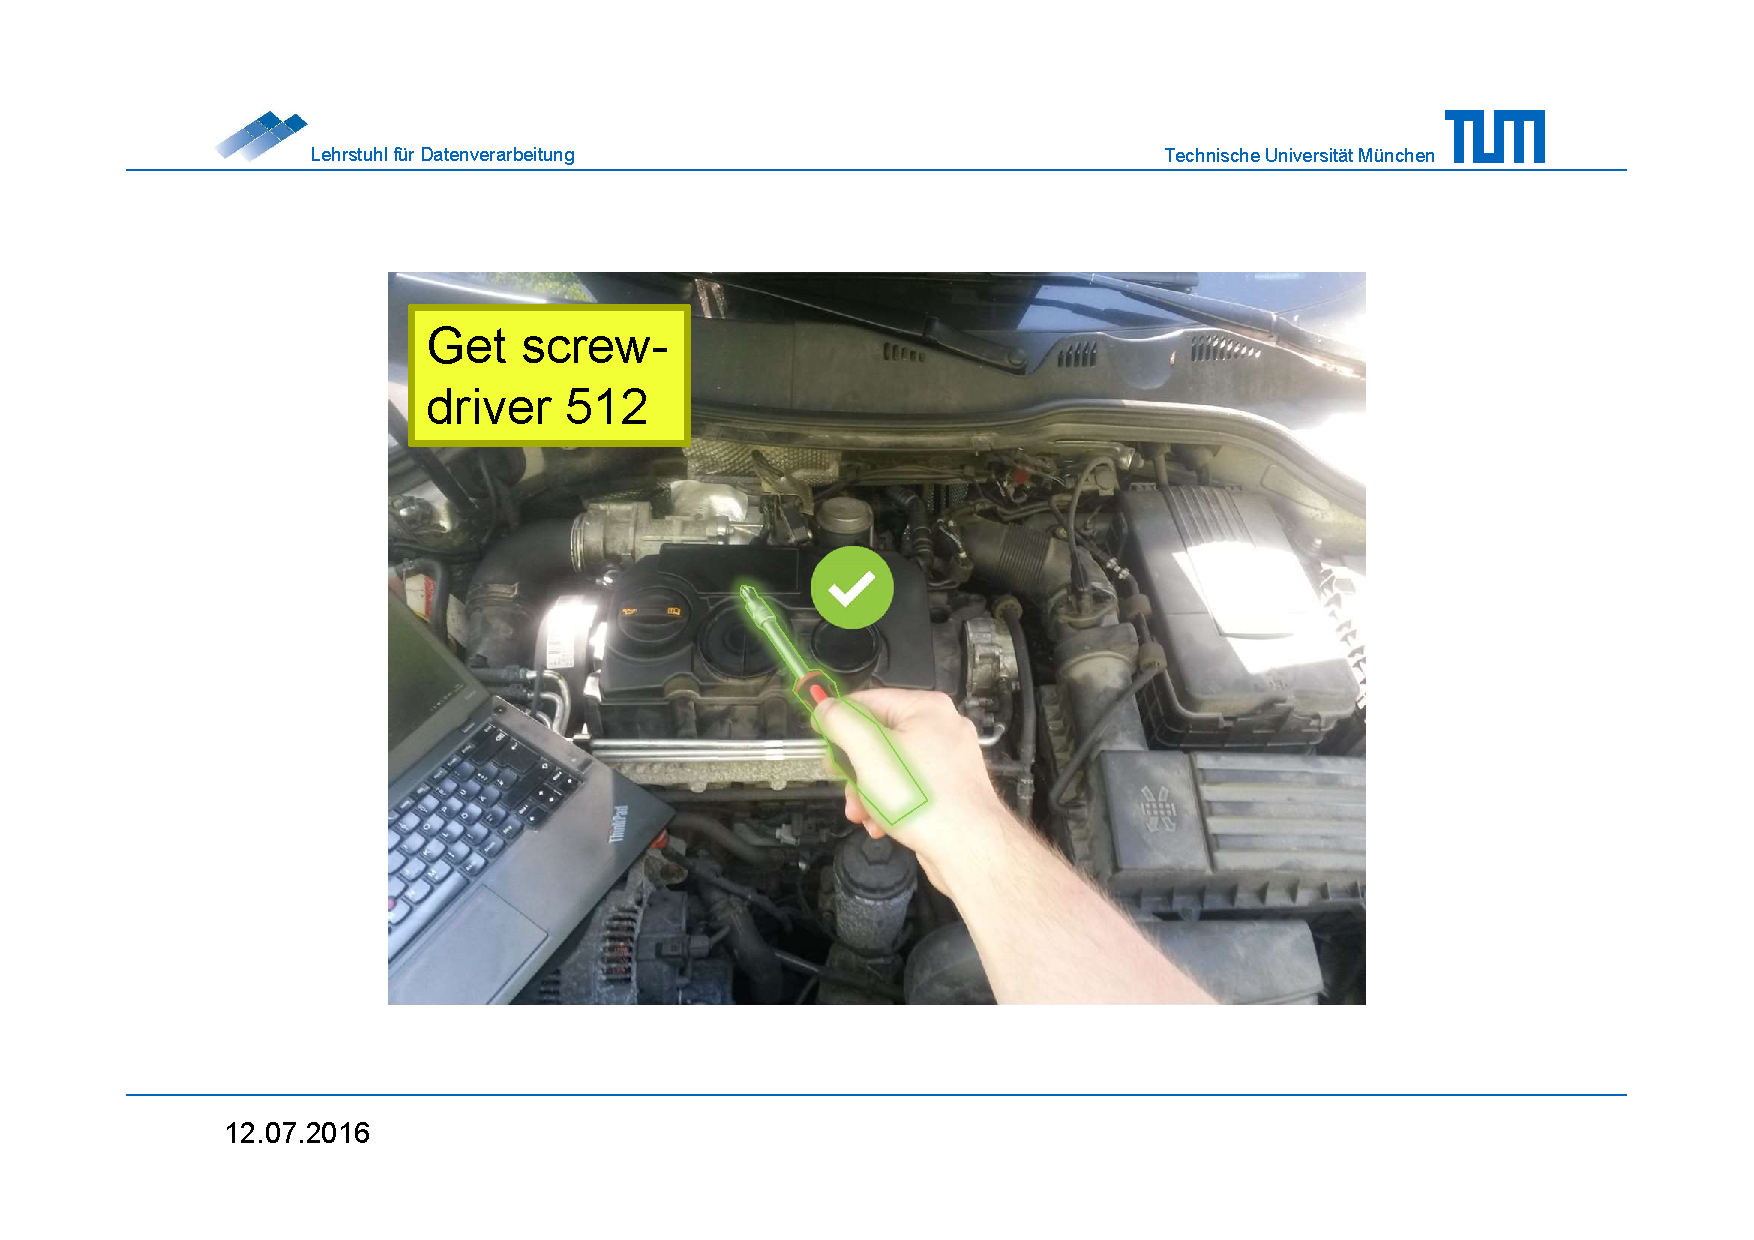
\includegraphics[width=\textwidth, trim=4cm 3cm 4cm 4cm, clip]{../images/instr-screwdriver.pdf}
			\centering
			\caption{Parties involved in the uFixit environment}
			\label{fig:instr-screwdriver}
		\end{figure}
		
		\autoref{fig:instr-hammer} and \autoref{fig:instr-screwdriver} show how one instruction step would look like. The necessary job to finish is shown in the top left - here: "Get screwdriver 512". When the user holds up a hammer, the AR device will register that and tell him that he is holding the wrong tool. After holding up the right tool, the manual will continue to the next step automatically.
		
	
	\section{Using existing AR hardware devices}
	
		One of the clous abouts uFixit is, the fixer can use almost every AR device on the market. It only has to fulfill a certain list of requirement that you can see in chapter 3. Although users will get the most excellent experience with AR head mounted devices like the Microsoft HoloLens or the Meta 2 (\autoref{fig:meta2}), other devices like smartphones are also supported.
		
		\begin{figure}[H]
			\centering
			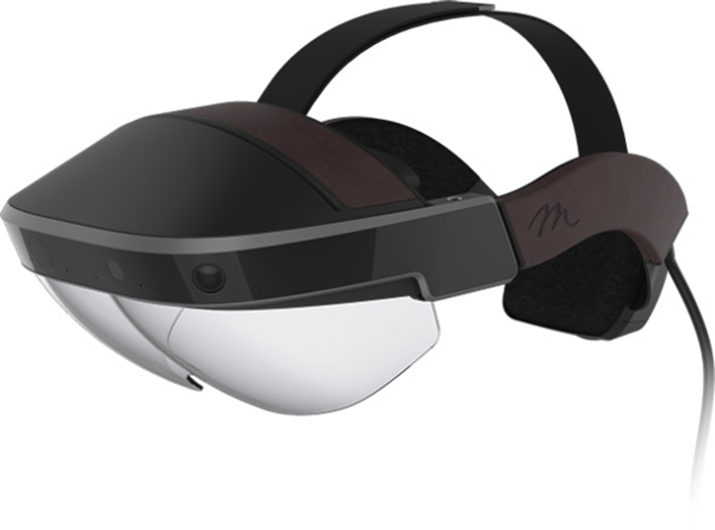
\includegraphics[width=0.5\linewidth]{../images/meta2.png}
			\caption{Meta 2 - Only one of the many devices uFixit will support}
			\label{fig:meta2}
		\end{figure}
		
		One outstanding example of this kind, which will receive special support, is Google's Project Tango. This is basically an augmented reality platform definition for Android based phones and tables.
		
		\begin{figure}[H]
			\centering
			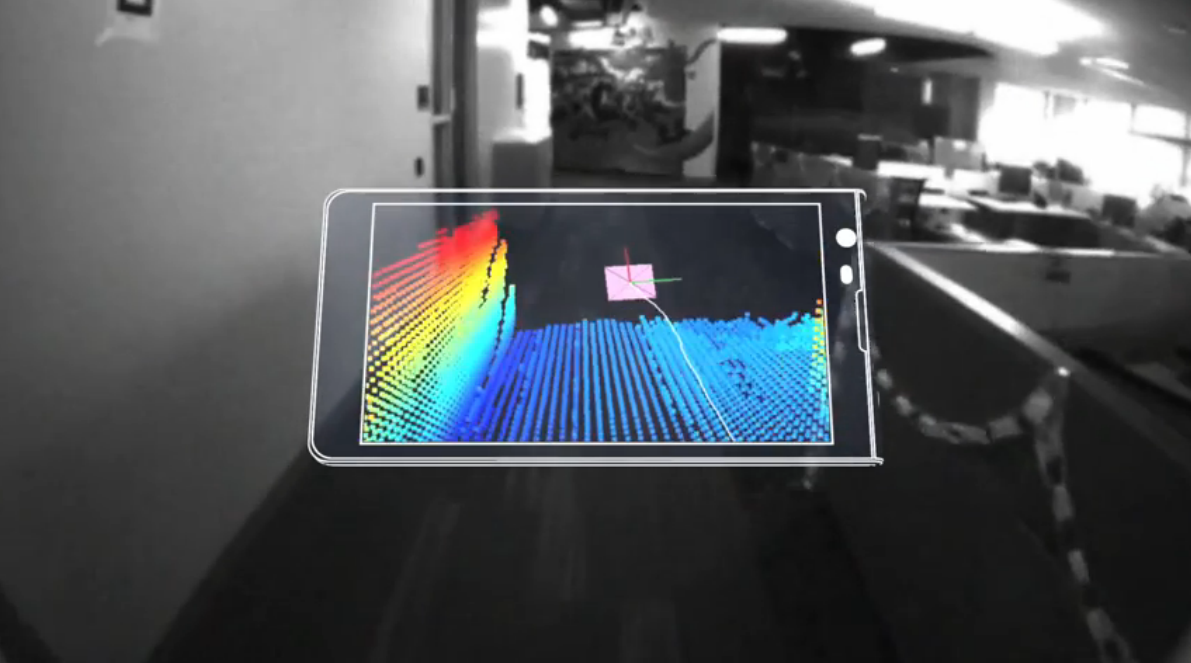
\includegraphics[width=0.7\linewidth]{../images/project-tango}
			\caption{Registration visualized using Project Tango by Google}
			\label{fig:project-tango}
		\end{figure}
		
		Of course if one does not have a suitable device, the manuals always can be watched using a webbrowser on out web portal as simple classical pages.
		
	
	\section{Software}
	
		To create the manuals we were talking about in \eqref{sec:instr-format}, we need special software. This will be the major products uFixit will ship. One are a plugins for a variety of well-established 3D CAD software which is already used to design the products. Before discussing this, the focus will be the other one: an application for the Experts that do not have special software but only the same devices as the end user.
	
		\subsection{Our gem: Community Manual Creation Software}
		
			- for everyone that owns an AR device
			
			- very intuitive, simple, fool proof
			
			- insert arrows by gestures, ...
	
		\subsection{3D CAD software for manufacturers}
		
			- needs good 3D model
			
			- can contain animations or see through content

			- complicated, only possible with previous training

		\subsection{Use tutorials on the device you like}
		
			- basically bring manual to as many devices as possible
			
			- classical screen
			
			- smartphones, tables with back camera
			
			- AR head mounted devices

	\section{Experts Motivation}
	
		uFixit relies heavily on the Fixers to get involved in the community and to start creating own manuals. This can solely be based on idealism. Believing this would work on the other hand is pretty naive. Our solution: Money!
		
		Many big software companies nowadays have something called bug bounty program. This means if a person finds a bug of a certain severity in the manufacturers product, he will get rewarded when reporting it. This is very convenient for the company considering they do not have to pay everyone that is searching for these flaws in the software.
		
		We want the same principle integrated into uFixit. Experts should be lured into a \textbf{manual bounty program} that will reward them every time a Fixer solves a problem using his tutorial. The money will come from the manufacturer who themselves do not have to pay for personal but rather only a small amount for high quality content.
	
	\section{Feedback}
	
		To provide the user with highest quality manuals, there will be an opportunity to rate each an every of them within a review system. Online shopping nowadays would be unimaginable without reviews just because no one likes to buy untested stuff. Especially when the end user needs quick and good help, he might invest in a manual that has a 100\% rating instead first trying the free to use 75\% one.

		\begin{figure}[H]
			\centering
			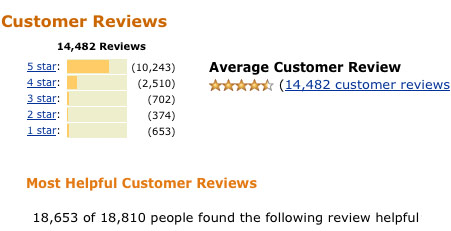
\includegraphics[width=0.7\linewidth]{../images/how-to-get-amazon-reviews-kindle.jpg}
			\caption{Example of product reviews on \url{amazon.com} with a overwhelming good average rating}
			\label{fig:amazon-reviews}
		\end{figure}
		
		\autoref{fig:amazon-reviews} is a screenshot from the \url{amazon.com} website. It shows a product review page with an overwhelming good average rating. Most of the users would now be convinced this is a great product and buy it without further research or thinking. the uFixit review system will be quite similar to this one because it will increase community involvement and building.
